\documentclass[border=10pt]{standalone}
\usepackage{tikz}
\usetikzlibrary{arrows.meta, shadings, positioning}

\begin{document}
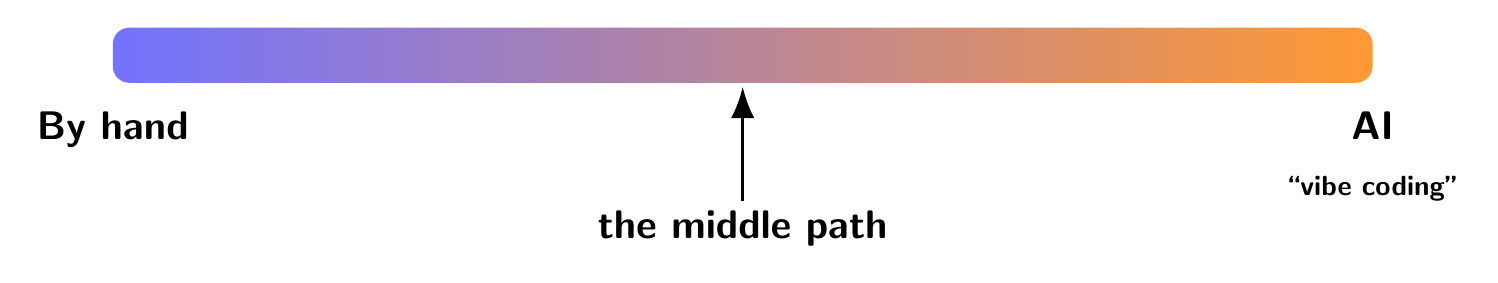
\begin{tikzpicture}[font=\sffamily]

  % Gradient spectrum bar.
  \shade[left color=blue!55, right color=orange!80, rounded corners=6pt]
    (0,0) rectangle (16,0.7);

  % Endpoint labels (below the bar).
  \node[anchor=north, font=\sffamily\bfseries\Large] at (0, -0.25)
    {By hand};
  \node[anchor=north, font=\sffamily\bfseries\Large, align=center] at (16, -0.25)
    {AI \\[2pt] \normalsize\itshape ``vibe coding''};

  % Middle annotation: label below + arrow pointing up to the bar.
  \node[anchor=north, font=\sffamily\bfseries\Large, align=center]
    (mid) at (8, -1.5) {the middle path};
  \draw[-{Latex[length=4mm, width=3mm]}, line width=1.2pt]
    (mid.north) -- (8, -0.05);

\end{tikzpicture}
\end{document}
